\documentclass[10pt,a4paper]{article}
\usepackage[margin=18mm]{geometry}
\usepackage[T1]{fontenc}
\usepackage{lmodern,graphicx,booktabs,amsmath,xcolor}
\usepackage{amssymb}
\usepackage[hidelinks]{hyperref}
\setlength{\parindent}{0pt}
\setlength{\parskip}{6pt}
\begin{document}
{\Large\bfseries An actual Jacobian elliptic-cover basis for C7}\par
23 November 2026 \quad Native correctness; unsigned [pcc:unverified]

\textbf{Outcome.} The actual degree-two/two/three elliptic covers give a
written degree-nine isogeny between the genuine genus-three Jacobian and
$E_7^3$. Native geometric-fibre push--pull checks agree on all eleven
rational elliptic points. This makes the cover correspondence concrete;
the integral CM19 map and an ECDLP computational advantage remain open.

\begin{center}
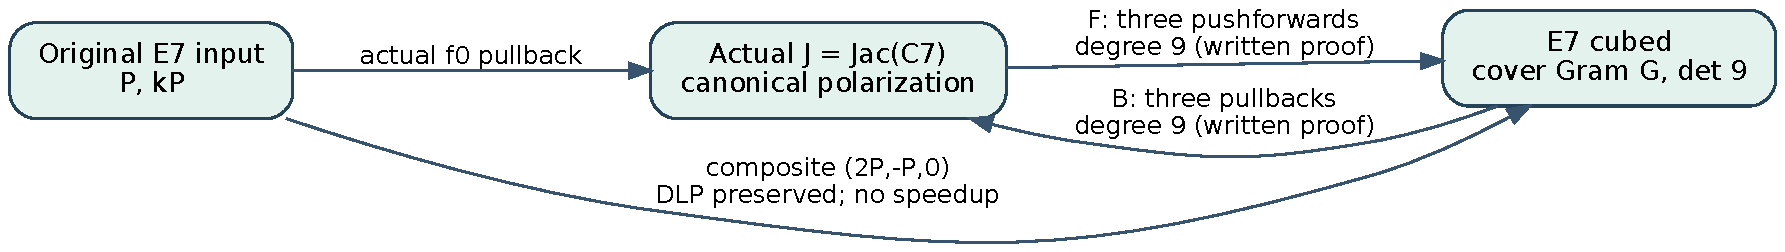
\includegraphics[width=\linewidth,height=58mm,keepaspectratio]{gram.pdf}
\end{center}

\textbf{Fixed actual maps.} Use $E_7:y^2=x^3+2x+6$ and
\[
 C_7:\ (Z^2+6X^2+3XY+Y^2)^2=Y(X^3+2XY^2+6Y^3).
\]
Let $f_0$ be the degree-two deck quotient, $f_1=f_0\circ R$ for the
qualified order-three projective automorphism, and $f_3$ the actual
degree-three quotient with its qualified elliptic model conversion.
Set $\phi_i=f_i^*:E_7\to J$, $B=(\phi_0,\phi_1,\phi_3)$, and
$F=B^\dagger$ using canonical polarizations. The global identity is
\[
 F B=G=\begin{pmatrix}2&-1&0\\-1&2&0\\0&0&3\end{pmatrix},
 \qquad \det G=9,\quad \deg B=\deg F=9.
\]

\textbf{Actual fibre qualification.} Every one of the eleven target points
has a full geometric fibre for each cover: square roots in
$\mathbb F_{49}$ for degree two, cube roots in $\mathbb F_{343}$ for
degree three. Each source point satisfies the original quartic, restores
the forward target and has the correct Frobenius-stable multiplicity.
Actual projective inverse charts also roundtrip.

\begin{center}
\begin{tabular}{lr}
\toprule
Observable & Full retained count\\
\midrule
Complete geometric fibres &33\\
Weighted geometric points &77\\
Entirely rational / extension fibres &25 / 8\\
Push--pull maps / rational images &9 / 99\\
Actual addition laws on computed images &1089\\
Missing-basepoint rejections / zero-offset positives &11 / 11\\
\bottomrule
\end{tabular}
\end{center}

\textbf{The basepoint is essential.} Compute each map as the actual elliptic
sum on $f_j^{-1}(P)$ minus the actual sum on $f_j^{-1}(O)$, with scheme
multiplicities. For $f_0$ the original infinity fibre is
$[1:0:1]+[1:0:-1]$, whose $f_3$ sum is $(1,3)$, not $O$.
Omitting it fails all eleven tested cross-map images. The zero-offset
degree-two diagonal is retained as an eleven-case positive control.

Full native source 746db916; unsigned data 1ce706. [pcc:unverified]
\newpage
{\Large\bfseries Global proof, real controls and remaining obstruction}\par

\textbf{Why the degree is global.} The finite cohort does not prove the
Jacobian identity. The separate written argument uses standard genuine
Jacobian push--pull/group-trace identities, Rosati positivity and ordinary
elliptic endomorphism theory. In normal coordinates
$[X:Y:Z]=[x+y+z:5x:y-z]$, the deck involution swaps $y,z$ and sends
the order-three quotient coordinate $w$ to $-w$. It acts by $[-1]$ on
the quotient Picard group, so the degree-two/three cross terms vanish.

The order-three trace then gives $h+\bar h=-2$ for
$h=\phi_0^\dagger R^*\phi_0$. Rosati Cauchy--Schwarz gives
$N(h)\le4$. The qualified elliptic trace is $-3$, with fundamental
discriminant $-19$, hence $\operatorname{End}(E_7)=\mathcal O_{-19}$.
For $\omega=\pi+2$,
\[
 N(a+b\omega)=a^2+ab+5b^2=(a+b/2)^2+19b^2/4.
\]
An element of norm at most four must be an integer, giving $h=-1$.
Together with the cover-degree diagonal, this proves $G$. Since
$\deg G=N(\det G)=81$ and dual isogenies have equal degree, $B,F$
have degree nine. They are separable and injective on two-primary and
eleven-primary torsion. The known rational orders $11^3$ on both sides
make $F:J(\mathbb F_7)\to E_7(\mathbb F_7)^3$ bijective.
This avoids the prior abstract rank-three Hermitian classification,
but is still a written proof with explicit standard dependencies,
without a compiled generic Mathlib theorem.

\textbf{Real ramification and infinity controls.} The two degree-three
ramified infinities have multiplicity three. Replacing that multiplicity
by one fails both the geometric degree and the actual elliptic push sum.
Swapping the quotient infinity images fails the actual positive-infinity
image. Pristine cases restore. No scalar/log label is supplied to any
curve-map or fibre constructor; no synthetic genus-three group is used.

\textbf{Execution and custody.} All seven strict C phases exit zero,
guards unchanged; Rust 1.99.1, warnings denied, overflow/debug assertions,
one worker, 120s/2GiB per phase. All 34 locked inputs were completely read
back before execution. Full stdout is 12923 bytes, SHA256
\texttt{0c42162a\ldots c84d69d}; all 38 small originals are retained.
The original 4599336-byte ELF is temporary custody-pending. The first
source-lock metadata defect and the 17469-byte first formatting negative
remain immutable. No old automorphism/H/field-triples driver was replayed.

\textbf{Next obstruction and cost standing.} The cover basis has Gram $G$,
not the identity polarization. Its integral gluing at three and relation
to CM19 $H$ must be constructed before transporting an arbitrary product
matrix to an integral Jacobian endomorphism. Actual nontrivial CM19
$S$/J4/target maps, independent replay and formal-library work remain.
The original input transfers to $(2P,-P,0)$, preserving DLP but providing
no new solve advantage. Same-prime-field covers give no subfield descent;
larger ambient Jacobian size does not beat the original elliptic reference.
Full cold costs need a separately promising mechanism first.

\href{https://github.com/isogeny-labs/crypto/tree/746db9161fe54d85a621a7303abe013fd2a33535/research/chained_cm19_jacobian_gram_20261123}{Frozen source/protocol/global written proof};
\href{https://github.com/isogeny-labs/crypto/tree/c875d22a619c363b3974a5d338943bf26de421f9/research/chained_cm19_jacobian_gram_20261123}{complete native result}.
KB/Conductor absent; no novelty clearance. Parent Hermitian raw approved
custody, paid STOP/vault/owners and CI/merge requirements persist.
[pcc:unverified]
\end{document}
